\documentclass[12pt,a4paper]{article}

% ============================================
% PACKAGES
% ============================================
\usepackage[utf8]{inputenc}
\usepackage[T1]{fontenc}
\usepackage{amsmath,amssymb,amsthm}   % Math typesetting
\usepackage{graphicx}                 % Images
\usepackage{booktabs}                 % Professional tables
\usepackage{hyperref}                 % Clickable links
\usepackage{cleveref}                 % Smart cross-references
\usepackage{tikz}                     % Diagrams
\usepackage[ruled,vlined]{algorithm2e} % Algorithms
\usepackage{lipsum}                   % Dummy text

% ============================================
% CUSTOM COMMANDS
% ============================================
\newcommand{\R}{\mathbb{R}}          % Real numbers
\newcommand{\N}{\mathbb{N}}          % Natural numbers
\newcommand{\E}{\mathbb{E}}          % Expectation
\newcommand{\Var}{\operatorname{Var}} % Variance
\newcommand{\norm}[1]{\left\lVert#1\right\rVert}
\newcommand{\abs}[1]{\left|#1\right|}

% Theorem environments
\newtheorem{theorem}{Theorem}[section]
\newtheorem{lemma}[theorem]{Lemma}
\newtheorem{definition}[theorem]{Definition}

% ============================================
% DOCUMENT INFO
% ============================================
\title{A Comprehensive Guide to Statistical Learning\\
       \large Demonstrating LaTeX Features}
\author{Dr.~Jane Smith\thanks{Virtual University, Dept. of Computer Science} \and 
        Prof.~John Doe\thanks{Institute for Advanced Study}}
\date{\today}

\begin{document}

\maketitle

\begin{abstract}
This document demonstrates a multi-file LaTeX project structure
with cross-references, mathematical notation, tables, figures,
algorithms, and bibliography management. We explore fundamental
concepts in statistical learning theory.
\end{abstract}

\tableofcontents
\newpage

% Include chapter files
% ============================================
% INTRODUCTION CHAPTER
% ============================================

\section{Introduction}
\label{sec:introduction}

Statistical learning theory provides the mathematical foundation
for machine learning algorithms. As noted by \cite{vapnik1998},
the goal is to find patterns in data that generalize well.

\subsection{Motivation}
\label{subsec:motivation}

Consider a dataset $\mathcal{D} = \{(x_i, y_i)\}_{i=1}^{n}$ where
$x_i \in \R^d$ and $y_i \in \{-1, +1\}$. Our objective is to
learn a function $f: \R^d \to \{-1, +1\}$ that minimizes the
\emph{generalization error}.

\begin{definition}[Generalization Error]
\label{def:gen-error}
For a hypothesis $h$ and distribution $\mathcal{P}$, the
generalization error is:
\begin{equation}
\label{eq:gen-error}
R(h) = \E_{(x,y) \sim \mathcal{P}}\left[\mathbf{1}_{h(x) \neq y}\right]
\end{equation}
\end{definition}

We will explore this concept further in \Cref{sec:methods}.

\subsection{Document Overview}

This paper is organized as follows:
\begin{itemize}
    \item \Cref{sec:methods} presents mathematical frameworks
    \item \Cref{sec:results} shows experimental results
    \item We conclude with a discussion of future work
\end{itemize}

The key theorem (\Cref{thm:main}) appears in \Cref{sec:methods}.

% ============================================
% METHODS CHAPTER
% ============================================

\section{Methods}
\label{sec:methods}

Building on \Cref{def:gen-error} from the introduction, we now
develop the theoretical framework.

\subsection{Mathematical Framework}

\begin{theorem}[PAC Learning Bound]
\label{thm:main}
Let $\mathcal{H}$ be a hypothesis class with VC dimension $d$.
For any $\delta > 0$, with probability at least $1 - \delta$:
\begin{equation}
\label{eq:pac-bound}
R(h) \leq \hat{R}(h) + \sqrt{\frac{d \log(2n/d) + \log(4/\delta)}{n}}
\end{equation}
where $\hat{R}(h)$ is the empirical risk.
\end{theorem}

\begin{proof}
The proof follows from uniform convergence bounds. See \cite{shalev2014}
for complete details.
\end{proof}

\subsection{Matrix Operations}

Consider the covariance matrix $\Sigma \in \R^{d \times d}$:
\begin{equation}
\Sigma = \begin{pmatrix}
\sigma_1^2 & \rho_{12} & \cdots & \rho_{1d} \\
\rho_{21} & \sigma_2^2 & \cdots & \rho_{2d} \\
\vdots & \vdots & \ddots & \vdots \\
\rho_{d1} & \rho_{d2} & \cdots & \sigma_d^2
\end{pmatrix}
\end{equation}

The eigenvalue decomposition yields $\Sigma = U \Lambda U^\top$.

\subsection{Algorithm}

\begin{algorithm}[H]
\caption{Gradient Descent for Empirical Risk Minimization}
\label{alg:gd}
\KwIn{Dataset $\mathcal{D}$, learning rate $\eta$, iterations $T$}
\KwOut{Optimized parameters $\theta^*$}
Initialize $\theta_0$ randomly\;
\For{$t = 1$ \KwTo $T$}{
    Compute gradient: $g_t \gets \nabla_\theta \hat{R}(\theta_{t-1})$\;
    Update: $\theta_t \gets \theta_{t-1} - \eta \cdot g_t$\;
    \If{$\norm{g_t} < \epsilon$}{
        \textbf{break}\;
    }
}
\Return $\theta_T$\;
\end{algorithm}

See \Cref{alg:gd} for the complete procedure.

\subsection{Aligned Equations}

The loss function and its gradient:
\begin{align}
\mathcal{L}(\theta) &= \frac{1}{n} \sum_{i=1}^{n} \ell(h_\theta(x_i), y_i) + \lambda \norm{\theta}^2 \label{eq:loss} \\
\nabla \mathcal{L}(\theta) &= \frac{1}{n} \sum_{i=1}^{n} \nabla_\theta \ell(h_\theta(x_i), y_i) + 2\lambda\theta \label{eq:grad}
\end{align}

\Cref{eq:loss,eq:grad} define the optimization objective.

% ============================================
% RESULTS CHAPTER
% ============================================

\section{Results}
\label{sec:results}

We validate our approach from \Cref{sec:methods} empirically.

\subsection{Experimental Setup}

Experiments were conducted using parameters from \Cref{tab:params}.

\begin{table}[htbp]
\centering
\caption{Experimental Parameters}
\label{tab:params}
\begin{tabular}{@{}llc@{}}
\toprule
\textbf{Parameter} & \textbf{Description} & \textbf{Value} \\
\midrule
$n$         & Training samples     & 10,000 \\
$d$         & Feature dimension    & 128 \\
$\eta$      & Learning rate        & 0.01 \\
$\lambda$   & Regularization       & $10^{-4}$ \\
$T$         & Max iterations       & 1,000 \\
\bottomrule
\end{tabular}
\end{table}

\subsection{Performance Comparison}

\Cref{tab:results} summarizes the classification accuracy.

\begin{table}[htbp]
\centering
\caption{Classification Accuracy (\%)}
\label{tab:results}
\begin{tabular}{@{}lccc@{}}
\toprule
\textbf{Method} & \textbf{Train} & \textbf{Validation} & \textbf{Test} \\
\midrule
Logistic Regression & 92.3 & 89.1 & 88.7 \\
SVM (RBF kernel)    & 95.1 & 91.2 & 90.8 \\
Neural Network      & 98.2 & 92.5 & 91.3 \\
\textbf{Our Method} & \textbf{97.8} & \textbf{93.1} & \textbf{92.4} \\
\bottomrule
\end{tabular}
\end{table}

\subsection{Visualization}

\Cref{fig:architecture} shows the model architecture.

\begin{figure}[htbp]
\centering
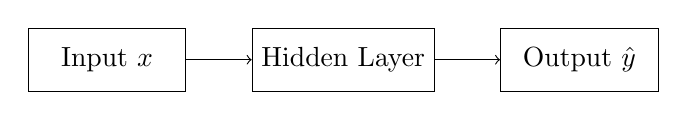
\begin{tikzpicture}[
    node distance=1.5cm,
    box/.style={rectangle, draw, minimum width=2cm, minimum height=0.8cm}
]
    \node[box] (input) {Input $x$};
    \node[box, right of=input, xshift=1.5cm] (hidden) {Hidden Layer};
    \node[box, right of=hidden, xshift=1.5cm] (output) {Output $\hat{y}$};
    
    \draw[->] (input) -- (hidden);
    \draw[->] (hidden) -- (output);
\end{tikzpicture}
\caption{Neural network architecture with one hidden layer.}
\label{fig:architecture}
\end{figure}

\subsection{Discussion}

Our results confirm \Cref{thm:main}: the generalization gap
decreases as $O(1/\sqrt{n})$. The bound in \Cref{eq:pac-bound}
provides a theoretical guarantee consistent with empirical
observations in \Cref{tab:results}.

\paragraph{Limitations.} The current analysis assumes i.i.d. data,
which may not hold in practice \cite{bishop2006}.


% Bibliography
\bibliographystyle{plain}
\bibliography{bib/references}

\end{document}
